\documentclass{article}

\usepackage{url}
\usepackage{tikz}
\usepackage{float}
\usepackage{amsmath}
\usepackage{enumitem}
\usepackage{graphicx}
\usepackage{xcolor,colortbl}
\usepackage[outdir=./]{epstopdf}

\usetikzlibrary{matrix, shapes, snakes, arrows}
\tikzset{>=triangle 45}

\title{CS 612: Assignment 3\\Summer 2014}

\author{Dustin Ingram}

\date{\today}

\begin{document}

\maketitle

\section*{Written}


\begin{enumerate}

\item{} % 1
Here, I am assuming that the goal is to maximize the received value in the util phase, and that the table for the utility function $U(x_1, x_2)$, where $x_1$ is the child and $x_2$ is the parent, is used as follows:

\begin{center}
\begin{tabular}{ |c|c|c|c| }
    \hline
            & $x_1^R$ & $x_1^G$ & $x_1^B$ \\\hline
    $x_2^R$ &  0 & 10 &  4 \\\hline
    $x_2^G$ & 10 &  0 &  1 \\\hline
    $x_2^B$ &  1 &  0 &  0 \\\hline
\end{tabular}
\end{center}

The messages sent will be as follows:\\

$D\rightarrow B:UTIL(B^R=10, B^G=10, B^B=1)$\\
$E\rightarrow B:UTIL(B^R=10, B^G=10, B^B=1)$\\
$F\rightarrow C:UTIL(C^R=10, C^G=10, C^B=1)$\\
$B\rightarrow A:UTIL(A^R=30, A^G=30, A^B=21)$\\
$F\rightarrow C:UTIL(C^R=20, A^G=20, A^B=11)$\\
$A\rightarrow B:VALUE(A^R)$\\
$A\rightarrow C:VALUE(A^R)$\\
$B\rightarrow D:VALUE(B^G)$\\
$B\rightarrow E:VALUE(B^G)$\\
$C\rightarrow F:VALUE(C^G)$\\

If minimization of the received value is the goal, any single-color coloring of the graph (all red, all blue, or all green) would result in a total minimum utility of zero.

\item{} % 2
\begin{enumerate}
\item{} % a

I would argue that if the individual processes operate on different, yet indistinguishable physical hardware, that it \emph{would not} be possible solve the leader election problem. I would assume that the different pieces of physical hardware operate at differing speeds, i.e., the hardware for process 1 was slightly faster than the hardware for process 2, resulting in asynchrony which would allow single process that arrived at a solution to the problem faster than its counterparts.

\item{} % b

If the machines now have GPS receivers attached to them, they now have a method to achieve clock synchronicity, and can split the execution time into slots for each process.

\end{enumerate}

\item{} % 3

Decentralized planning may not be a suitable approach if agents are self-interested. If there is potential for conflict, and no ability to resolve said conflict, no central authority to decide between two plans, and agents who do not act in the best interest of the ecosystem, deadlock is possible, and a group of agents may not be able to agree on a plan. The advantage, however, to a decentralized approach would be the lack of a single point of failure.

\item{} % 4

In this paper, Lamport realizes that describing a consensus algorithm in terms of a fictional Greek parliamentary body might have been too much for most people to understand. Instead, he attempts to describe the algorithm in plain English. The goal of the algorithm is to accept a single value from a group of proposed values by participators in the voting process. Participators are broken down into three classes of agents: proposers, acceptors, and learners. Proposers make multiple proposals of potential values to be selected. Any proposal can be abandoned by a proposer at any time, but usually this would happen when an acceptor indicates that they have already seen a better proposal. He goes on to provide an implementation of said distributed system as a deterministic state machine.

\begin{enumerate}

\item{} % a

The algorithm is not suitable when Byzantine failure can occur because the vanilla Paxos algorithm depends on the accuracy of the proposals and acceptances. If these messages are corrupt, inconsistent or incorrect, the algorithm has no way to compensate for this level of failure, and would not perform correctly.

\item{} % b

The Paxos algorithm can be extended to support Byzantine failure by including an additional ``Verify'' message. This message is sent between acceptors after receiving a proposal to verify it's accuracy.

\end{enumerate}

\end{enumerate}

\newpage

\section*{Programming}

For this problem, I wanted to examine the ``Ants Forage'' simulation, which is essentially an ant colony optimization problem. Specifically, I wanted to discover if there was a relationship between the number of food items an ant colony of a fixed size could collect over a set amount of time, and the evaporation rate (which is on a scale of 0.00 to 1.00). After some initial observations, I hypothesized that that there would be a "peak" evaporation rate at an evaporation rate of approximately 0.90, and that a higher evaporation rate would not necessarily correspond to a greater number of foods gathered.

For the experiment, I ran 1000 iterations of a simulation with 100 ants in the default environment for 3000 steps. The evaporation rate varied from 0.00 to 1.00 at increments of 0.01.

The resulting data and graph (below) disproved my hypothesis. In fact, foods gathered is linearly proportional to the evaporation rate. The highest evaporation rate (1.00) corresponded to the most foods gathered, on average. The data produced the linear function for foods given evaporation rate:

    $$ F(\delta_e) = 712.34\delta_e + 9618.16 $$

The graph is as follows, with a plot of all experimental data, as well as $F(\delta_e)$:

\begin{figure}[H]
\centering
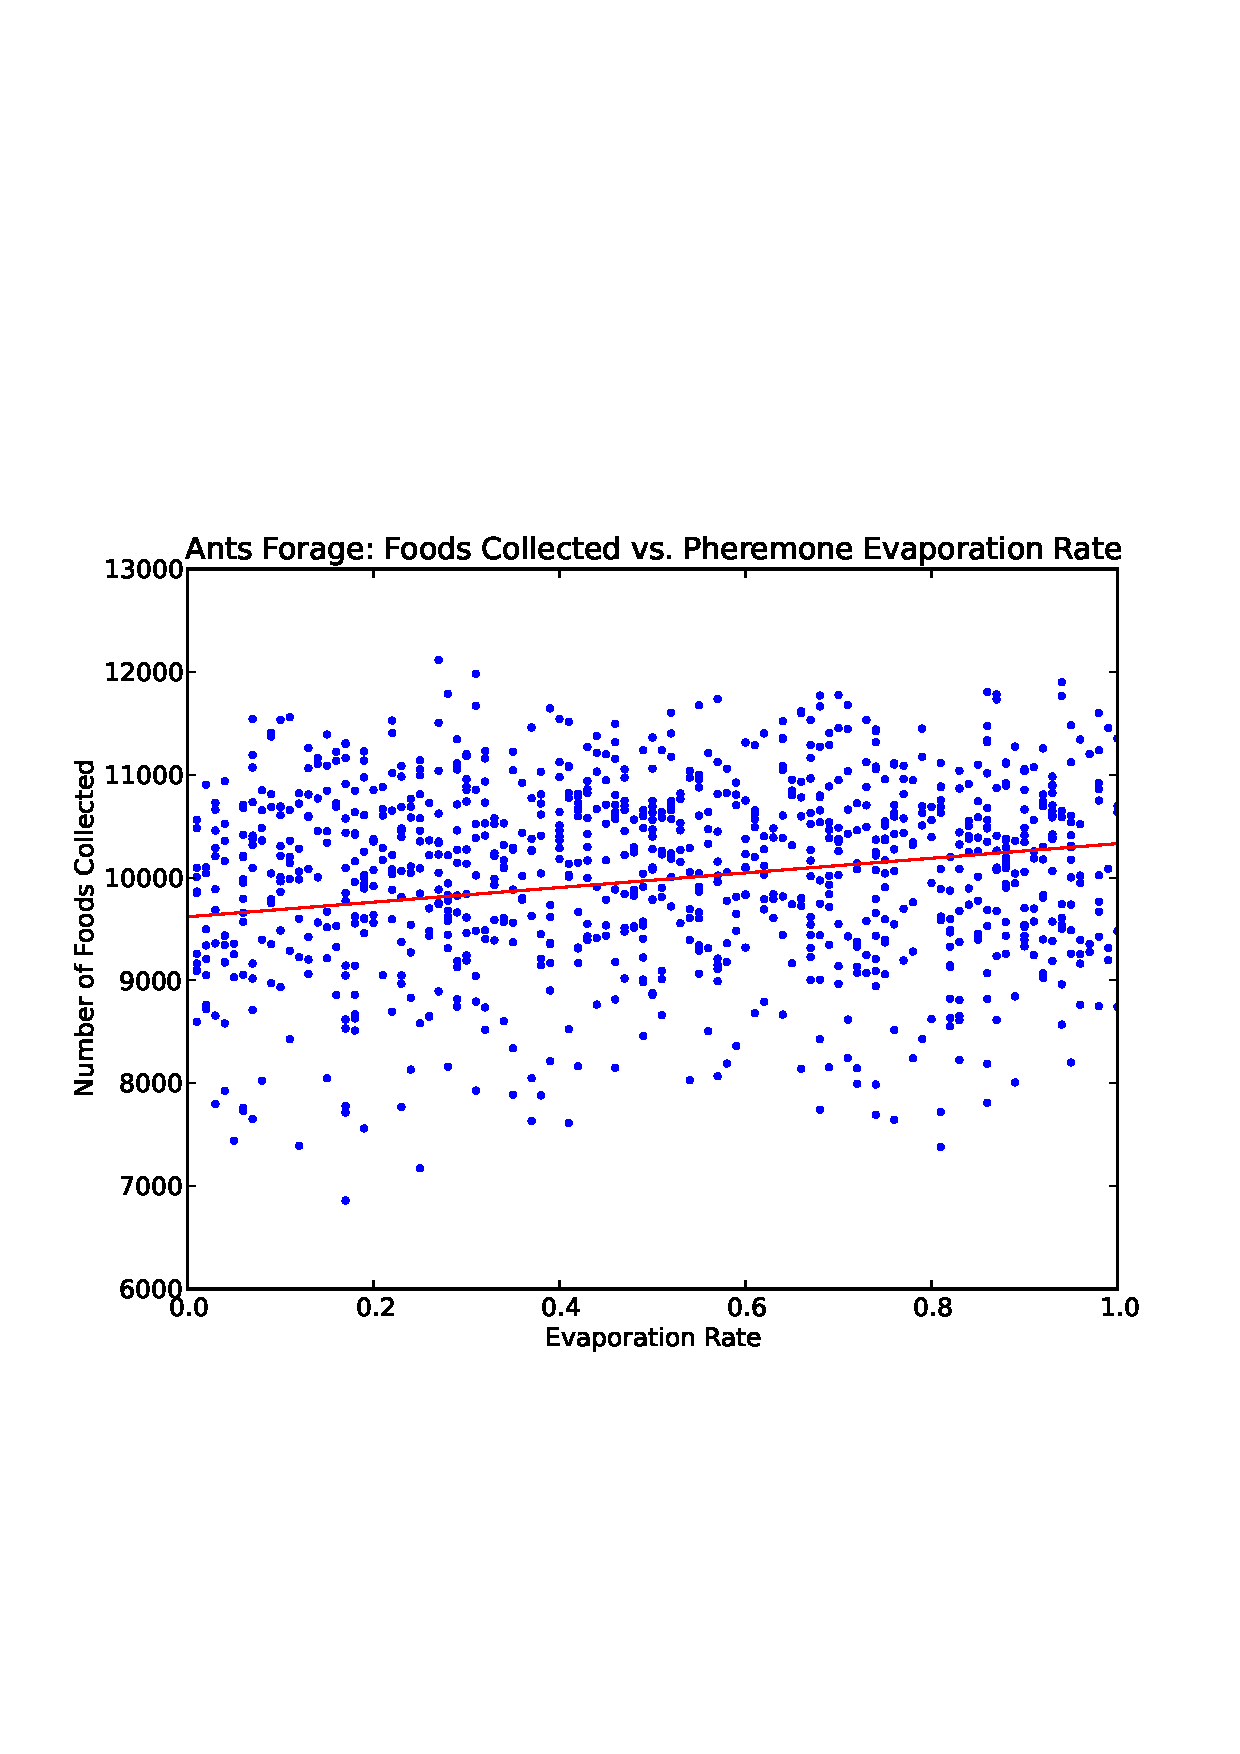
\includegraphics[width=\textwidth]{figs/a3}
\caption{Evaporation Rate vs. Foods}
\end{figure}



\end{document}
